\clearpage
\section{4 ПРИНЦИПИАЛЬНЫЕ ОГРАНИЧЕНИЯ}
Помимо выявленных проблем, которые необходимо решить при внедрении технологии в полноценный движок, у Nanite выявлены принципиальные ограничения:
\begin{itemize}
    \item оценка искажения не зависит от направления взгляда;
    \item невозможность анимации меша;
    \item невозможность автоматической децимации некоторых мешей.
\end{itemize}

\subsection*{Оценка искажения}
Оценка искажения мешлета зависит от расстояния до камеры, но не от направления взгляда.
В некоторых случаях искажение меша имеет разное значение с разных ракурсов, например, на кирпичной стене выравнивание зазоров между кирпичами будет куда более заметно, если смотреть почти параллельно стене, чем если смотреть перпендикулярно стене.
В классическом подходе к уровням детализации этим фактором пренебрегают.

\subsection*{Анимация}
При любом движении вершин друг относительно друга оценки искажения мешлетов окажутся некорректными, а описывающие объёмы мешлетов изменятся.
Из-за этого становится невозможным гарантировать сохранение свойства графа, на которое завязана отрисовка.
Поэтому технология Nanite работает только со статичными мешами: скалы, здания, статуи.
Это приводит к необходимости оставлять значительную часть сцены в классических уровнях детализации.

\subsection*{Автоматическая децимация}
Некоторые типы мешей, используемых в компьютерных играх, не являются поверхностями замкнутого объёма.
Синтетическим примером такого меша является плоский квадрат, представляющий из себя изначально сетку 64 на 64 малых квадрата.
Рёбра на периметре этого квадрата считаются входящими в шов в любом мешлете, из-за этого они никогда не подвергаются децимации, и квадрат оказывается невозможно уменьшить до 2 мешлетов, как видно на рисунке~\ref{fig:plane-1}.
\begin{figure}[h]
    \centering
    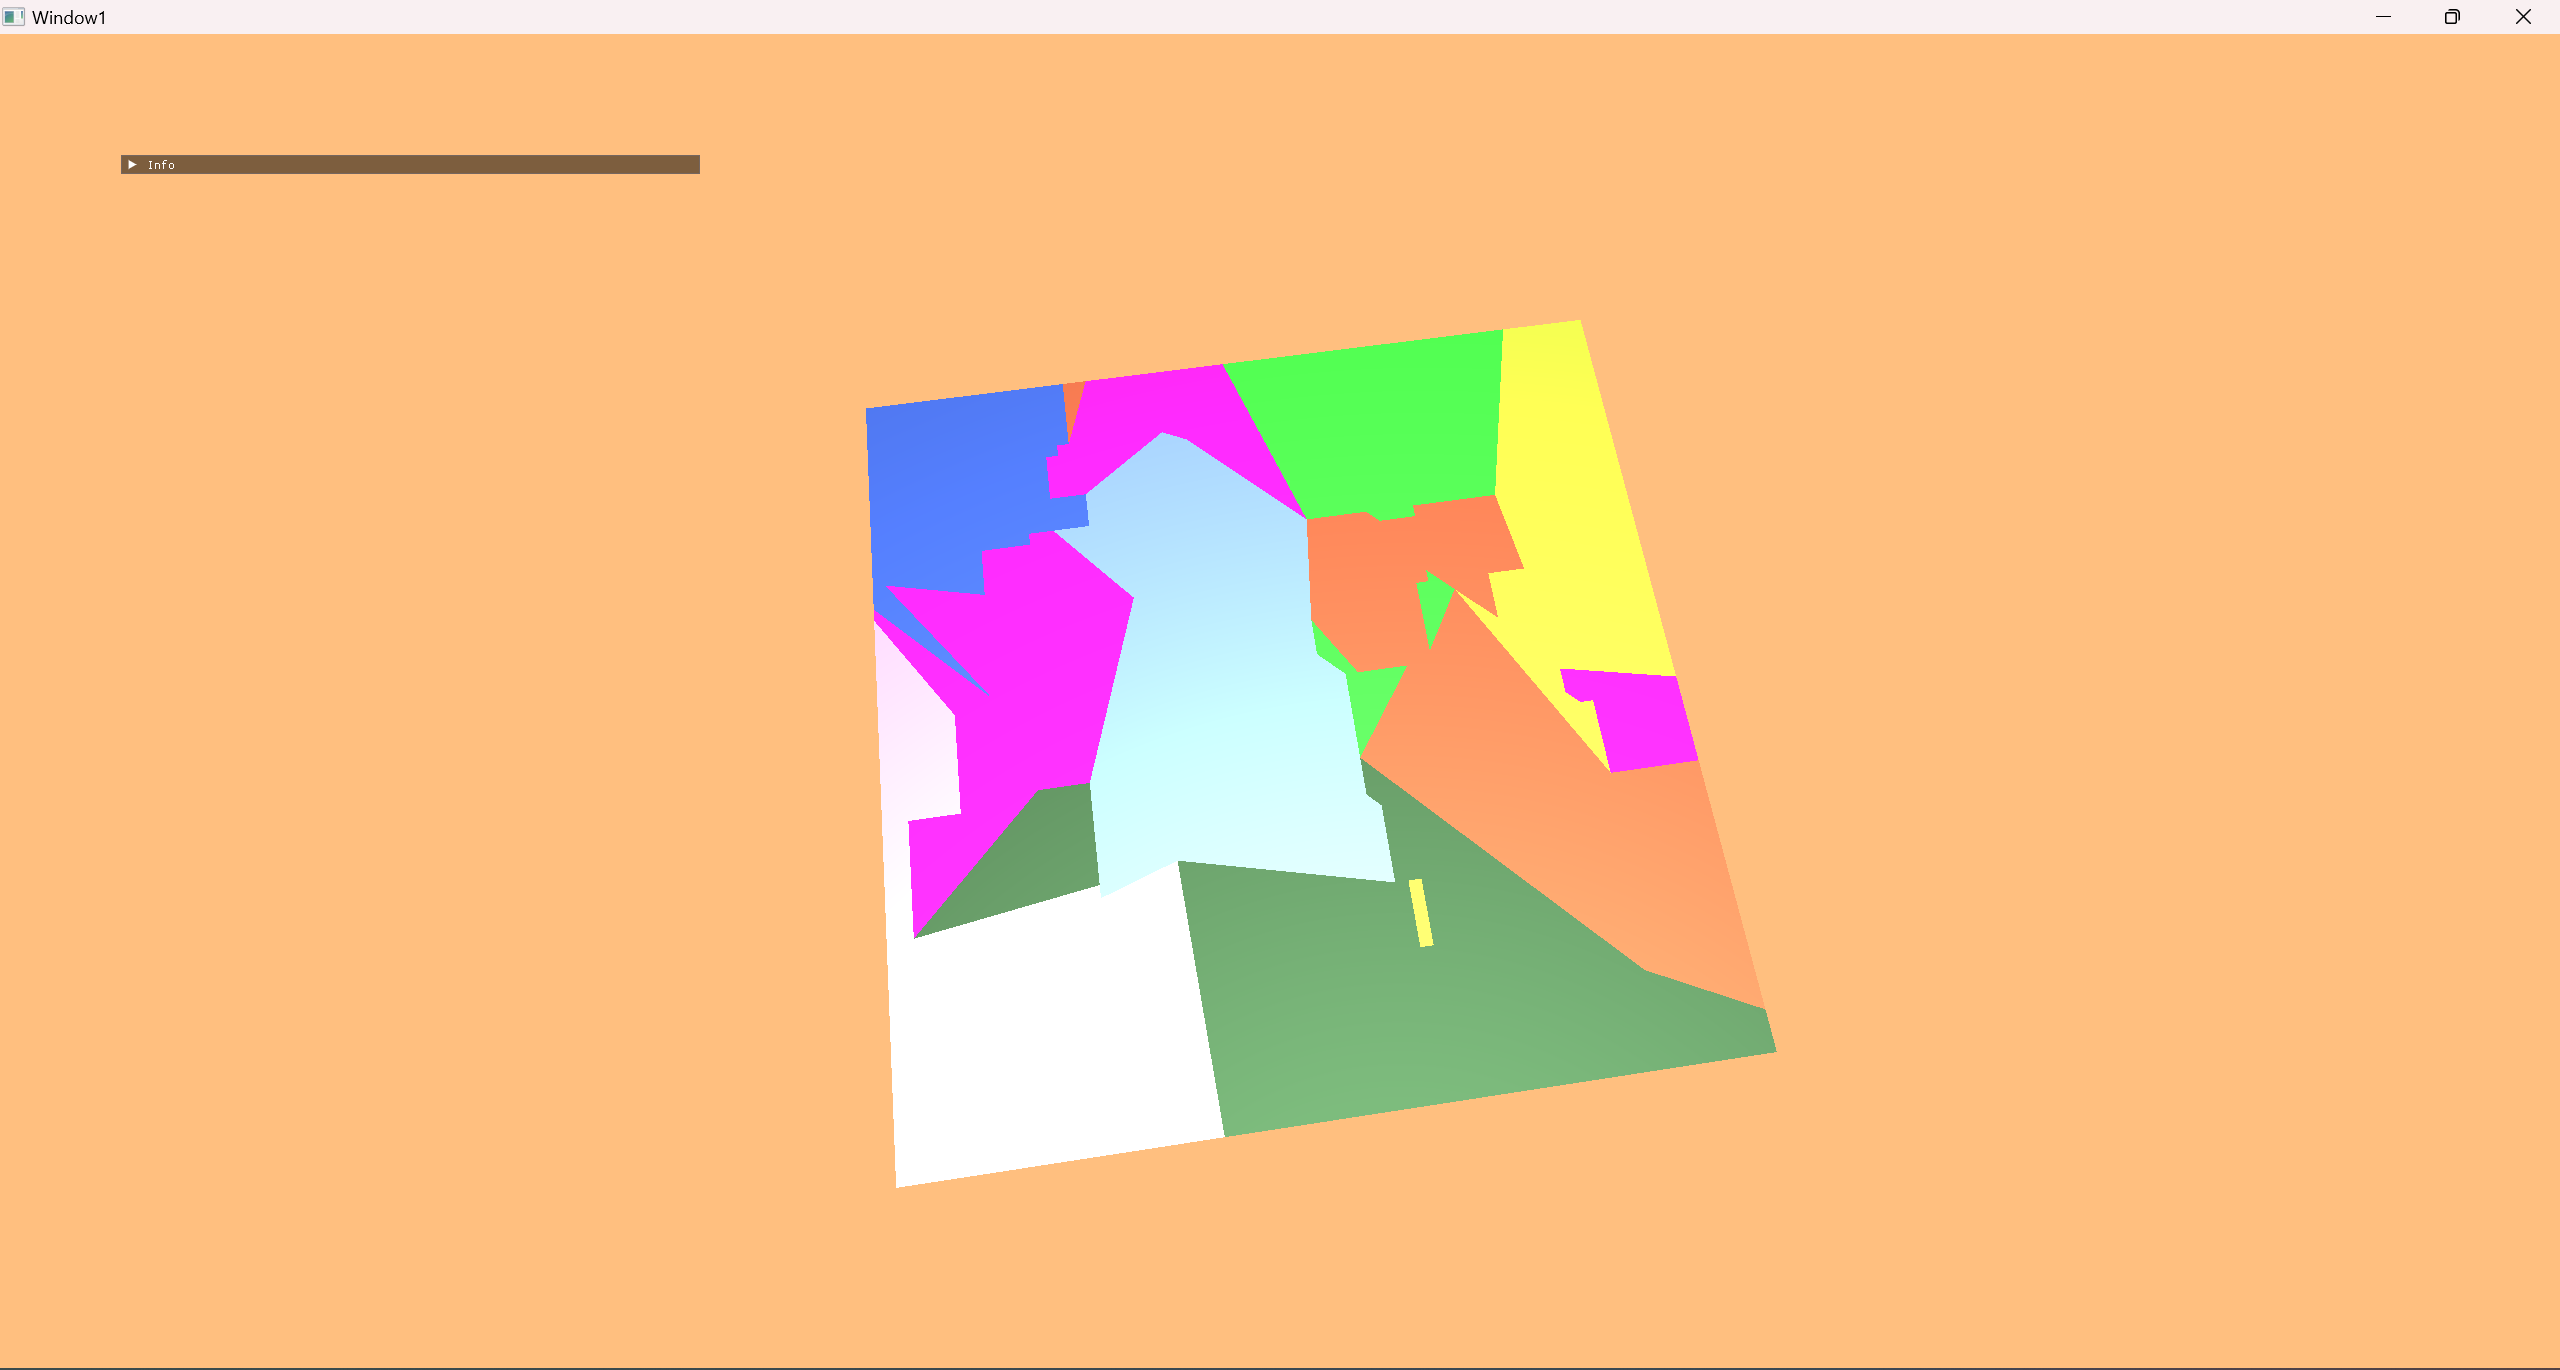
\includegraphics[width=\textwidth]{plane1.png}
    \caption{Плоскость}
    \label{fig:plane-1}
\end{figure}

В компьютерных играх существуют более естественные примеры таких мешей, не поддающихся децимации подобными алгоритмами, самый простой пример --- листва деревьев.
